\section{Experimental Methods}
\subsection{Photon Beam}
% ToDo: Think about if/where to include the calculation of the ratio of knockout neutrons to fission neutrons. Have only done calculation for Thorium.
A bremsstrahlung photon beam is produced by the passage of 10.5 MeV electrons through a 1" thick slab of aluminum.
Aluminum was chosen for a radiator because it has a neutron knockout threshold above the energy of the electron beam.
This ensured that the bremsstrahlung radiator would not be a source of fast neutrons which would have the potential to make their way into the experimental cell and cause false neutron events.
Downstream from the bremsstrahlung radiator, a sweeping magnet removes excess electrons from the photon beam (see figure~\ref{fig:Facility}).
Before reaching the experimental cell, the beam must travel through a series of polyethylene and lead collimators aimed at eliminating beam contaminants.
The energy distribution of photons that reach the target was assessed using an MCNP simulation which included the creation and collimation of the bremsstrahlung photons.
The resulting energy distribution is shown in figure~\ref{fig:BremDist}.

\begin{figure}[h]
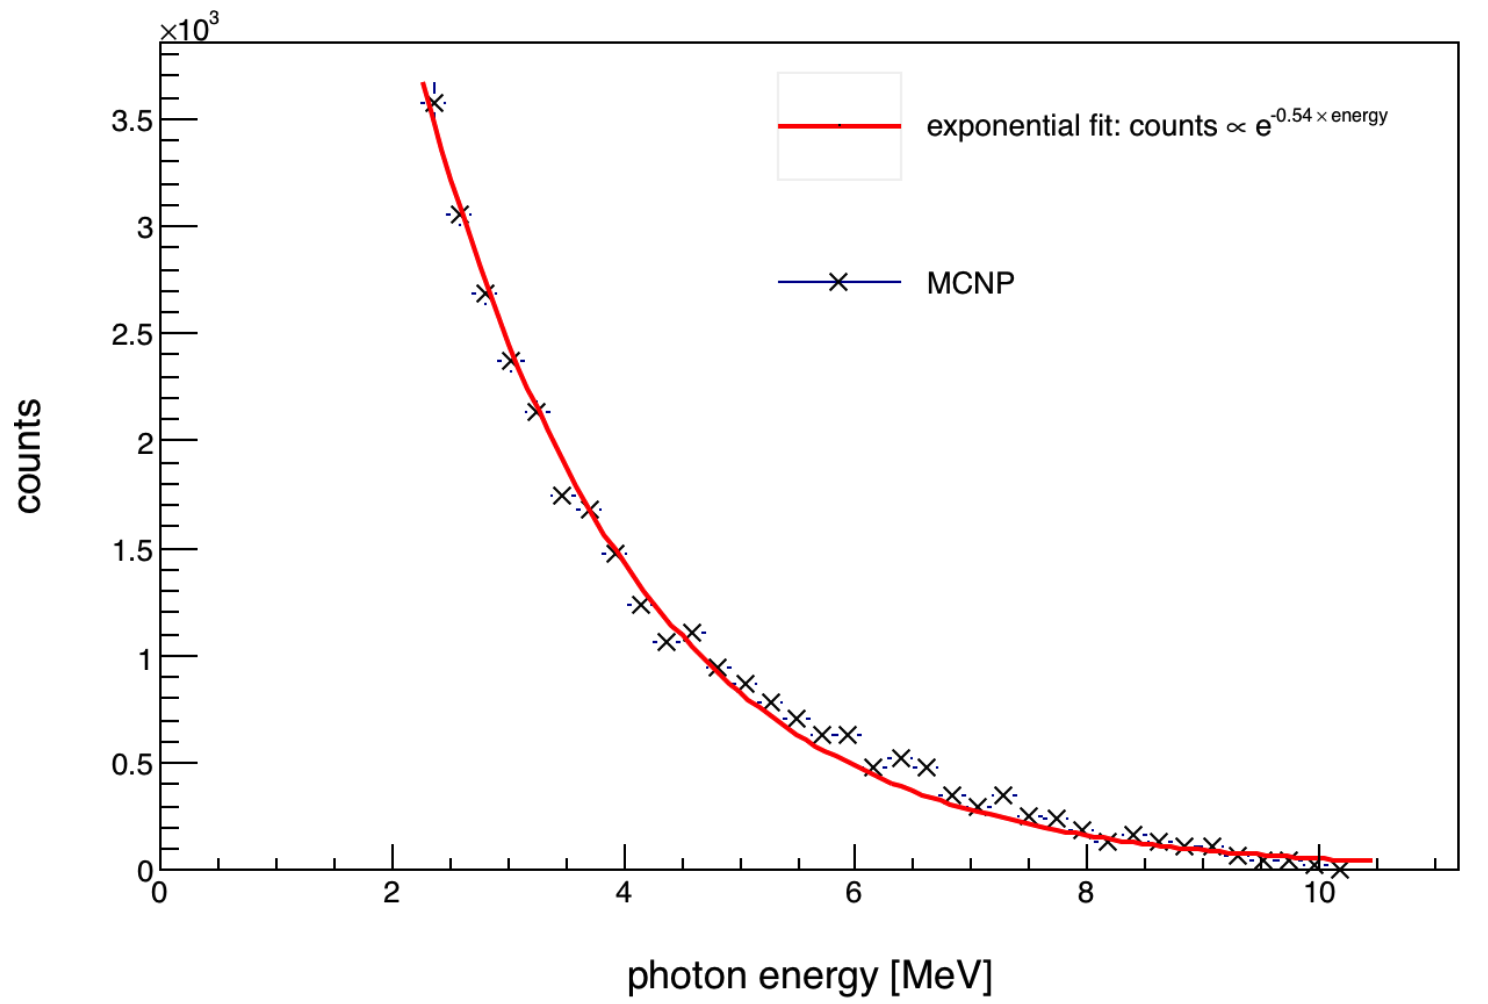
\includegraphics[width=0.9\textwidth]{Content/Methods/MCNPBremDistribution.png}
\caption{Energy distribution of the photons that reach the target, taken from an MCNP simulation of the production and collimation of the Bremsstrahlung beam.
The points are from the simulation. The line is an exponential fit of the form $Ae^{-bx}$.
The constant of proportionality, $A$, is arbitrary. The value for $b$ is 0.54.}
\label{fig:BremDist}
\end{figure}

When attempting a measurement of prompt neutrons from photofission, an ambiguity can arise between neutrons from photofission and neutrons from $(\gamma, xn)$.
This is because the two reactions have similar cross-sections within the GDR region.
Furthermore, there is significant overlap between the energy spectra of the neutrons from $(\gamma, xn)$ and those from photofission.
Because this measurement is concerned only with observing two neutrons in coincidence, it suffices to set the Bremsstrahlung end-point at 10.5 MeV, since this value is below the target's ($\gamma, 2n$) threshold of $\sim$12 MeV.
Despite setting the end-point below the ($\gamma, 2n$) threshold, there is still the possibility of detecting multiple neutrons from ($\gamma, 1n$) in a single pulse, which is referred to as an accidental coincidence.
An \textit{accidental} neutron coincidence occurs when two uncorrelated neutrons are detected in the same pulse.
The rate of accidentals follow the Poissonian distribution, setting them apart from correlated events, and as a result accidentals can be subtracted from the data.
The details and justifications for this procedure are discussed in section~\ref{Subtraction of Accidentals}.

The electron pulse width was set to 3 ns and had a 1.1A peak current, with a repetition rate of 240 Hz.
The 3 ns pulse width is not a large source of error in the measurements of neutron time of flight, since neutron events had a median time of flight of about 80 ns.
The accelerator's current is set by requiring that there be, on average, fewer than one fission per pulse in order to diminish the detection of accidentals.
% ToDo Discussion about the LINAC's low duty factor??

\subsection{Particle time of flight determination}
\label{reconstruction}
Each scintillator was equipped with two PMTs, one fixed at each end of the scintillation cell, with the exception of the detectors located farthest downstream at $\pm30^{\circ}$ which had a single PMT.
The reason for this difference is that, in order to diminish dead-time, the detectors at $\pm30^{\circ}$ were segmented to create two independent detectors.
A non-scintillating light-guide was fixed between each PMT and the scintillator to create 10 cm of space in order to allow scintillation light produced at the far end of the cell to have a change of reaching the PMT.
Each PMT provides a signal in response to scintillation light with a timing resolution of less than 2 ns.
The main source of uncertainly in the time of a particle hit is the variation in the time taken for scintillation light to propagate to the PMTs.
The time of events in the PMTs was always taken relative to a signal provided by the accelerator at the beginning of each pulse, referred to as the \textit{beam gun}.
Time of flight (ToF), the time for a particle to travel from the target to the face of a detector, was used to distinguish between photons and neutrons, and to measure neutron energy.
Scintillation light that is detected by the PMTs has a measured effective index of refraction of 3.
Consequently, there can be up to an 8 ns delay between the moment a particle scintillates in the detector and the time at which the scintillation light reaches a PMT.
The effective index of refraction is found by measuring the time taken for scintillation light to travel the full length of the detector.
The actual index of refraction of the material is about half that value, a difference which is the result of light rays bouncing from the walls of the scintillator on their way to a PMT.
The time of flight was calculated by taking the average between the times of signals in the top and bottom PMTs, and then subtracting a calibration offset.
In taking the average, there is a reduction in the sensitivity of the result to the variation of propagation times as a function of the position at which the particle scintillated.
This cannot be done in the detectors located at $\pm30^{\circ}$, because they have only one PMT.
However, since they are 1/3rd the length of the rest, scintillation light takes at most only 2.5 ns to propagate to the PMT, which is a tolerable amount of random error.
See section~\ref{Errors} for a deeper discussion of experimental errors.

The ToF of a particle causing coincident events in both PMTs of a detector obeys the following relationship:
\begin{displaymath}
ToF = C_i + \Delta t_{\text{avg}} 
\end{displaymath}
where $\Delta t_{\text{avg}} $ is the average between the timing from the top and bottom PMTs, and $C_i$ is a constant timing offset which is the same for every pulse.
The subscript on $C_i$ is used because the timing offset can be different for each detector.
Any process that produces a timing delay that does not change from pulse to pulse contributes to $C_{i}$.
Examples of this are: \begin{enumerate*}[font={\color{red!50!black}\bfseries}]
\item the time required for photons to travel from the bremsstrahlung radiator to the target
\item the propagation of signals through the wires connecting the PMTs
\item delays in the electronics for processing and
\item the transit time in the PMTs.
\end{enumerate*}

The time required for scintillation light to travel through the detector, from the point of scintillation to a PMT mounted at either end, can vary from 1 ns for particles that hit very close to a given PMT, to about 8 ns for particles that hit across the detector from a given PMT.
The sum of the times taken for scintillation light to travel to the top and bottom PMTs is just the time taken for the light to travel the full length of the detector.
The rate at which light propagates along the length of a detector is dependent on speed of light in the material and the light's flight path.
The flight paths of detected scintillation light tend to be parallel to the long axis of the detector, because these are the shortest paths possible, and only the first signal from a PMT is accepted.
Therefore, in taking the average of the times in the top and bottom PMT, the sensitivity of the result to the varying times required for the propagation of scintillation light is greatly reduced.
However, because the scintillation light does not always take to most direct path to a PMT, there is still some variation in the average scintillation propagation times.
This variation was measured using a $^{60}$Co source, which emits coincident photons.
The $^{60}$Co source is placed at several positions along the face of a lead shielded scintillator.
At each position, a small hole is drilled through the lead to give the $^{60}$Co source a line-of-sight to a well defined point on the scintillator.
A high timing-resolution photon detector is placed next to the $^{60}$Co source.
When the $^{60}$Co source decays, emitting two photons simultaneously, one photon is detected by the high timing-resolution detector serving as the ``start'' time, and the other photon scintillates in the detector being calibrated.
The times of signals from each PMT, taken relative to the start trigger, are averaged.
The photons from $^{60}$Co cause scintillation at a specified location, so variation remaining in the result is due to varying paths taken by the scintillation light, and is a reflection of the error in ToF measurement.
These results can be seen in figures~\ref{fig:Co60Validation} and~\ref{fig:Co60ValidationProject}.
% **ToDo: Make a figure for the setup of the co60 calibration.
\begin{figure}[H]
    \centering
    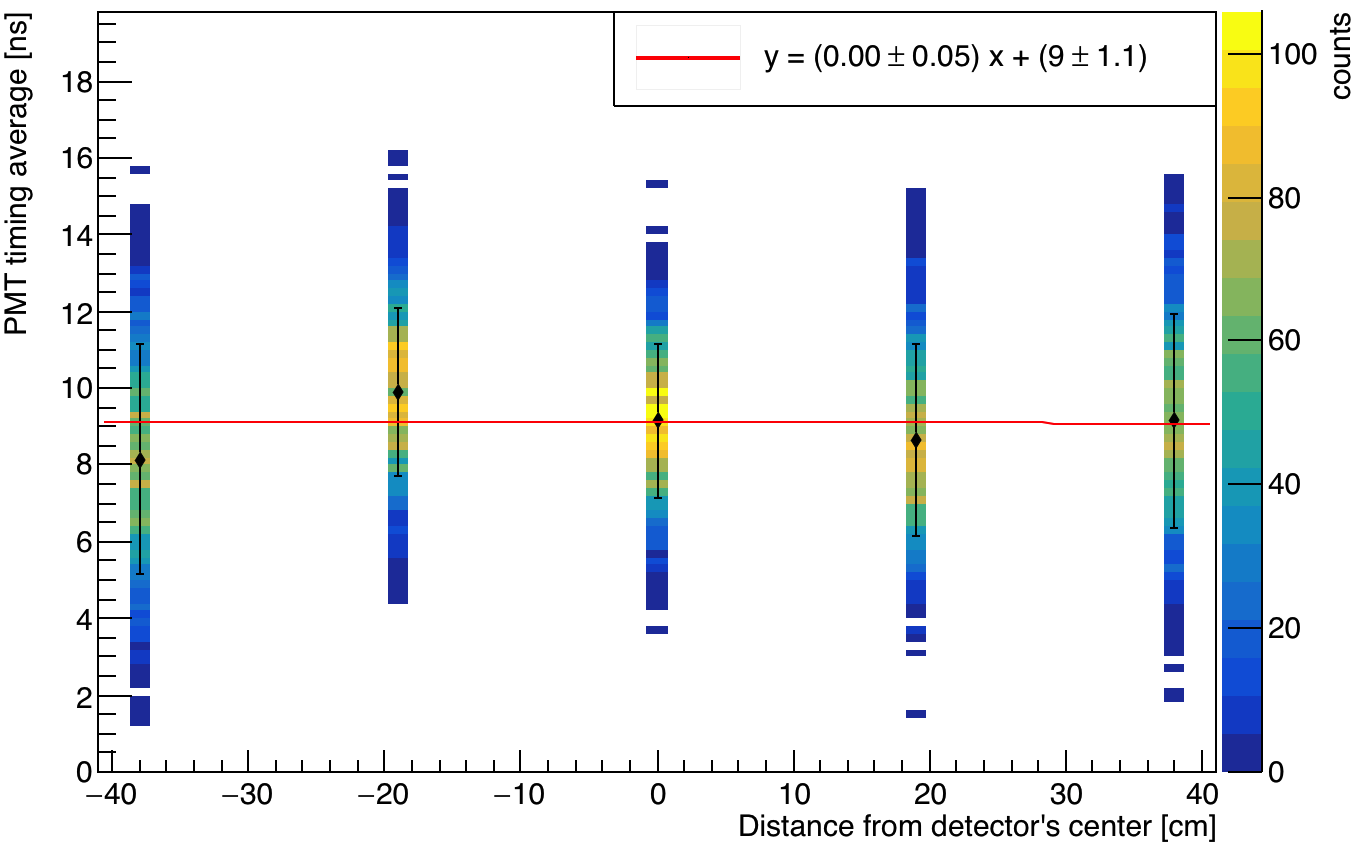
\includegraphics[width = 0.9\textwidth]{Content/Methods/CO60Validation.png}
    \caption{A $^{60}$Co source, which emits coincident photons, is placed at several positions along the face of a lead shielded scintillator.
    At each position, a small hole is drilled through the lead to give the $^{60}$Co source a line-of-sight to a well-defined point on the scintillator.
    Then, a high timing resolution photon detector is placed close to the $^{60}$Co source.
    When the $^{60}$Co source decays, emitting two photons simultaneously, one photon is detected by the high timing-resolution detector serving as the ``start'' time, and the other scintillates in the detector being calibrated.}
    \label{fig:Co60Validation}
\end{figure}
\begin{figure}
    \centering
    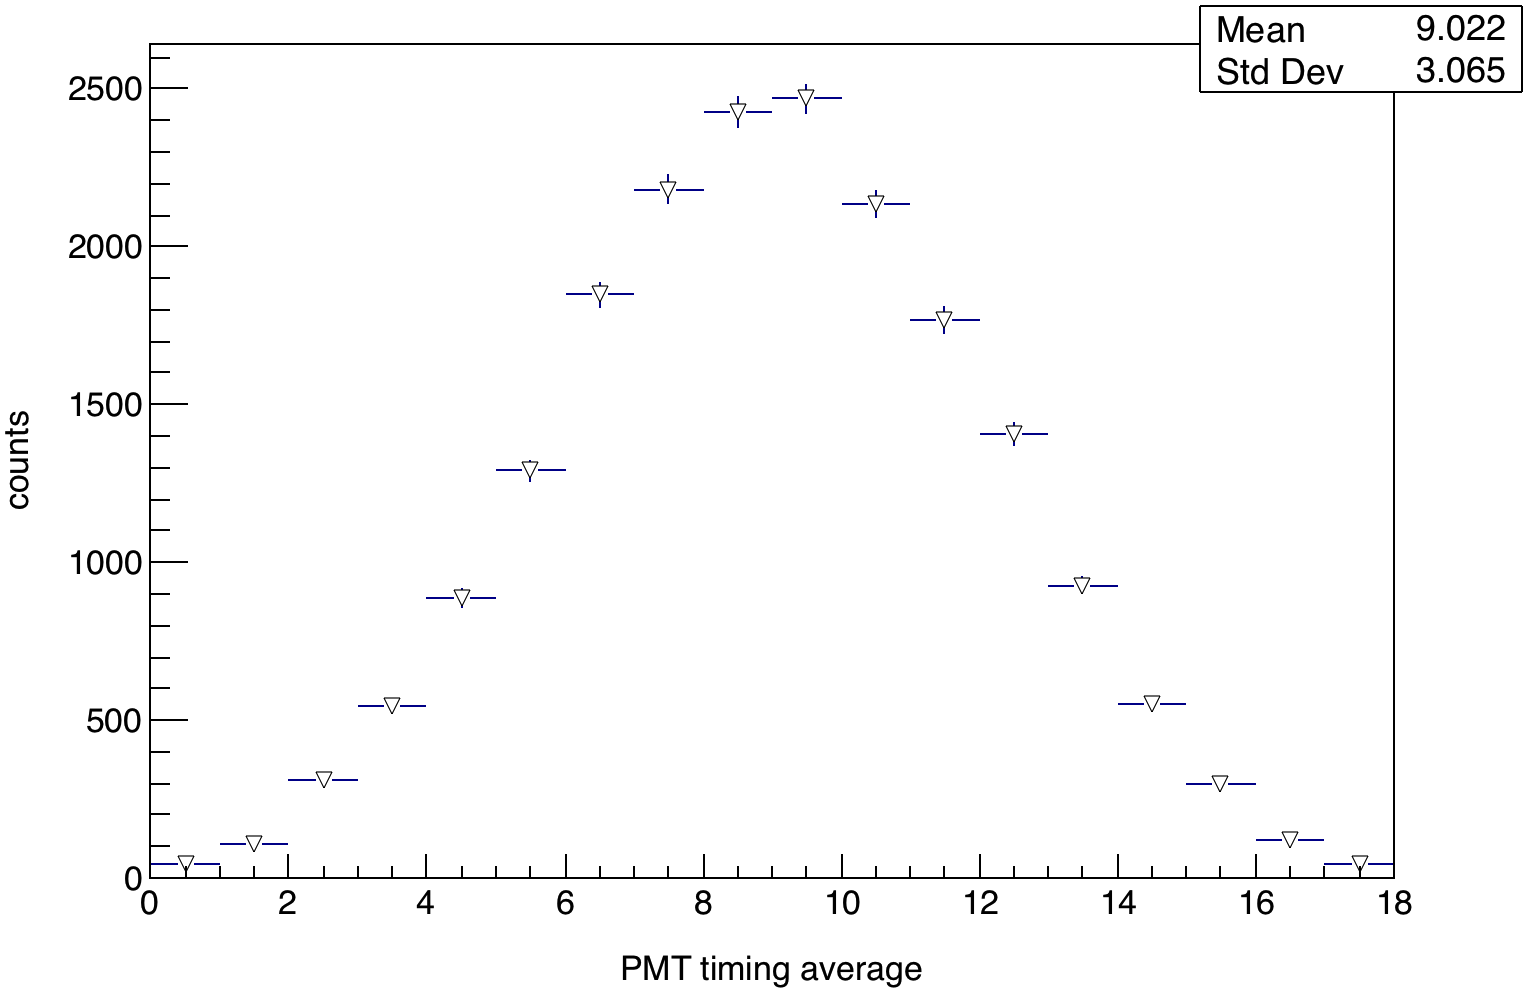
\includegraphics[width = 0.9\textwidth]{Content/Methods/CO60ValidationProject.png}
    \caption{Average of times in the top and bottom PMTs.
    Ideally, scintillation light would always take the same amount of time to travel the length of the detector, producing a delta function in this plot.
    This is not the case, however, because scintillation light doesn't always take the direct, shortest path to a PMT.
    Thus, the 3 ns standard deviation of this curve represents a source of error in the ToF measurement.
    These data, taken during calibration using a $^{60}$Co, are the same data used for fig~\ref{fig:Co60Validation}, projected onto the y-axis.
}
    \label{fig:Co60ValidationProject}
\end{figure}

The value of the constant offset for ToF calculation is determined by observing photons that scattered from the target.
Comparing the timing spectra of a non-neutron producing target made from aluminum, to the spectra produced when no target is used reveals a prominent peak caused by the scattering of photons from the target.
Aluminium does not produce photo-neutrons because the beams's Bremsstrahlung end-point is below Aluminium's ($\gamma$, n) threshold.
Photons scattered from the target must travel between 125 cm to 130 cm to reach a face of a detector, depending on whether the photons reach the detector near the center or at the edge.
It takes light 4.0 ns and 4.3 ns to travel 125 cm and 130 cm, respectively.
The difference between these two times is negligible for these purposes, so the ToF of photons that scatter from the target is assumed to be 4 ns.
With this assumption, the location of the photon peak in the timing spectra can be used to calculate the offset in each detector.
See figure~\ref{fig:ToFDetermination} for an illustration of this process.
%python file: ProductionAnalysis/TOFGraphs
\begin{figure}[htbp]
\begin{center}
\subfloat[$\Delta T$s with no target in place. ]{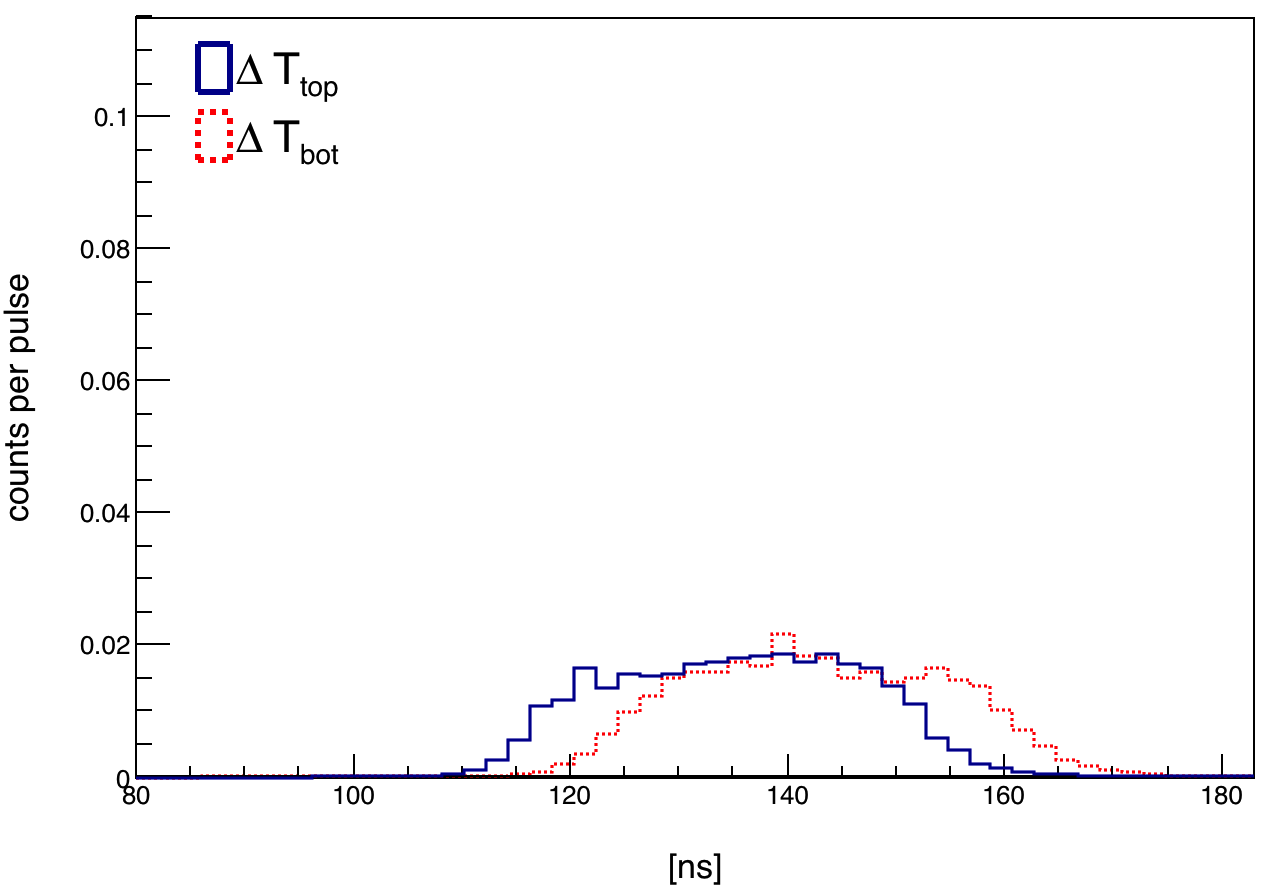
\includegraphics[width=0.5\textwidth]{Content/Methods/ToF0.png}}
\end{center}

\subfloat[$\Delta T$s with Aluminum target.]{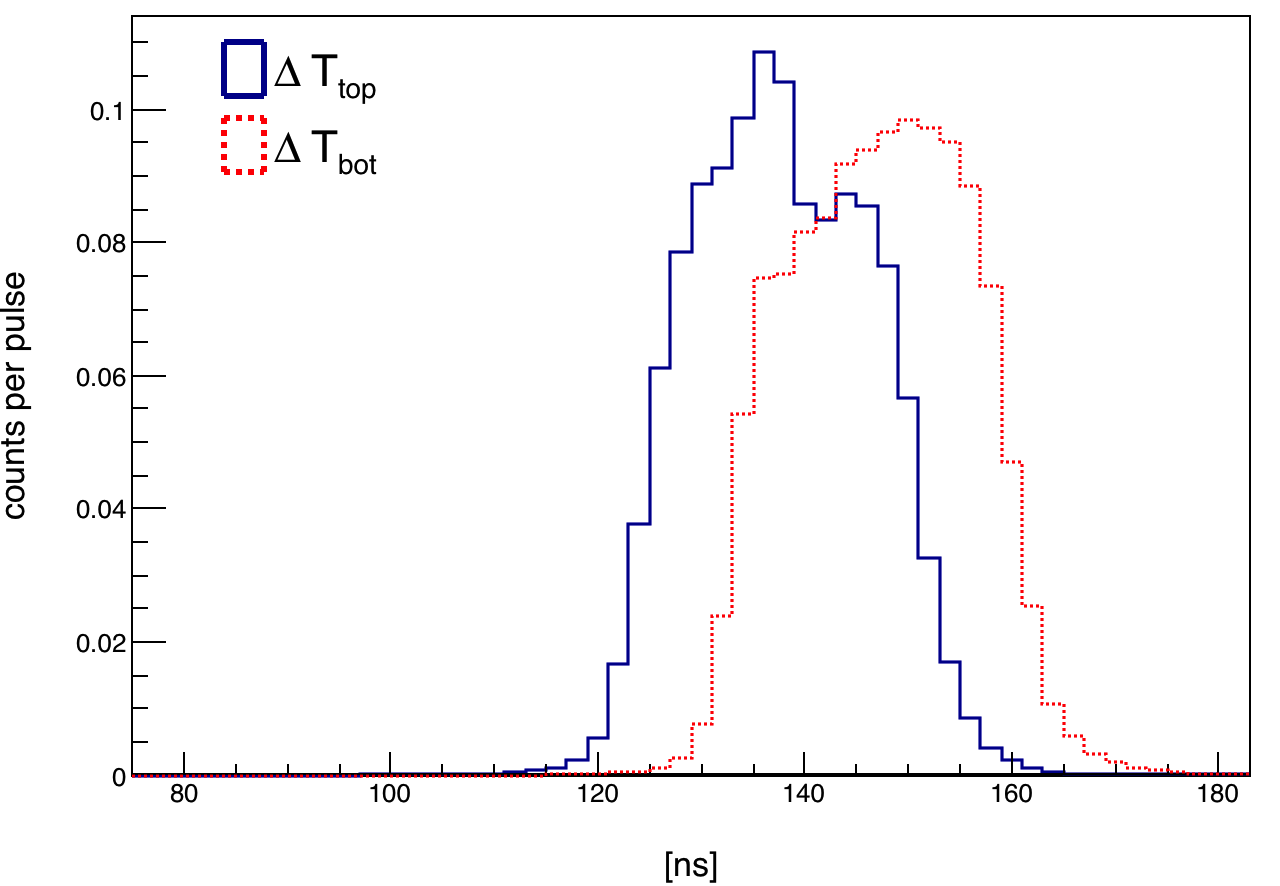
\includegraphics[width=0.5\textwidth]{Content/Methods/ToF1.png}}
\subfloat[Average of $\Delta T_{\text{top}}$ and $\Delta t_{\text{bot}}$  with Aluminum target in place.]{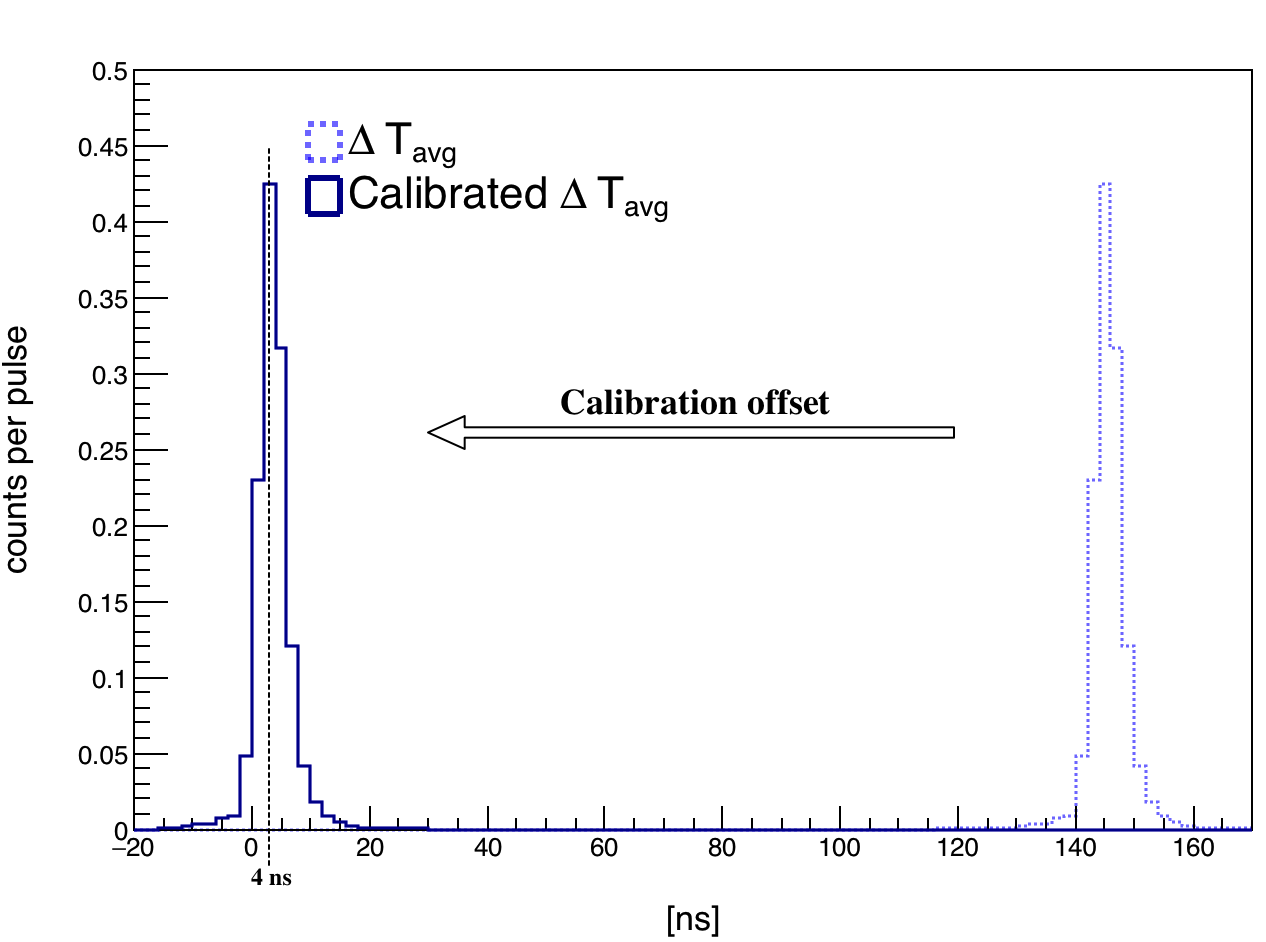
\includegraphics[width = 0.5\textwidth]{Content/Methods/ToF2.png}}
\caption{(a) $\Delta T$ spectra from each PMT of a detector with no target in place.
The beam dump is not able to collect all excess photons, so there is a background despite the lack of a target to scatter photons into the detectors.
The background is caused by photons that scatter from various surfaces within the experimental cell.
(b) The introduction of a non-neutron producing target made from aluminum produces a peak caused by the scattering of photons from the target.
These photons have a constant time of flight, so the width of these spectra are reflective of the range of times taken for scintillation light to propagate from the points of scintillation to a PMT.
(c) Taking the average between the $\Delta T$s of the top and bottom PMT gives a sharper peak, since the sum of times from both PMTs is a reflection of the time required for light to travel the entire length of a detector, regardless of the location of the particle hit.
The correct timing offset can be now be found since the photons have a time of flight of 4 ns. }
\label{fig:ToFDetermination}
\end{figure}
   
\subsection{Particle Position Reconstruction}
% ToDo: The determionation of position could use a figure. The figure could indicate verticle reconstruction, and horizontal error. 
Spacial resolution in the horizontal plane is determined by the physical dimensions of the detector.
The geometric center of a detector is used for the position, in the horizontal plane, of a particle hit.
The detector's dimensions in the horizontal plane are comparatively small at 3.8x15 cm$^2$, so in doing this, a positional uncertainty of $\pm$7.5 cm is introduced, which expressed in terms of an angle is $\pm4^{\circ}$.
The final results of this work use an opening angle bin width of 20$^{\circ}$, so $\pm4^{\circ}$ is not large enough be a cause for concern.
The largest contributor to uncertainty in particle position is the position in the vertical direction, which is determined by the timing difference between signals in the top and bottom PMTs.

The determination of a particle's position in the vertical direction relies on the timing of coincident signals from both the PMTs of a detector.
The timing difference obeys a linear relationship with respect to the location of the particle hit along the length of the detector.
The z-coordinate will hereafter refer to a particle's position along the vertical axis, where $z=0$ corresponds to the geometric center of the detectors.

As discussed before, detected scintillation light tends to take fairly direct paths to the PMTs, experiencing few reflections off the boundary of the scintillation cell.
As a result, the timing difference between signals in the top and bottom PMTs is proportional to the difference in path lengths that the scintillation light must travel to reach each PMT, which is in turn proportional to the z-coordinate of the particle hit.
The exact linear relationship is determined through calibration by using collimated photons from a $^{60}$Co source.
Calibration is achieved by measuring the PMT top-bottom timing difference while the $^{60}$Co source is fixed at five different locations along the detectors length.
The setup for calibration was discussed in section~\ref{reconstruction}.
The result is shown in figure~\ref{fig:PMTDifference}.

\begin{figure}
    \centering
    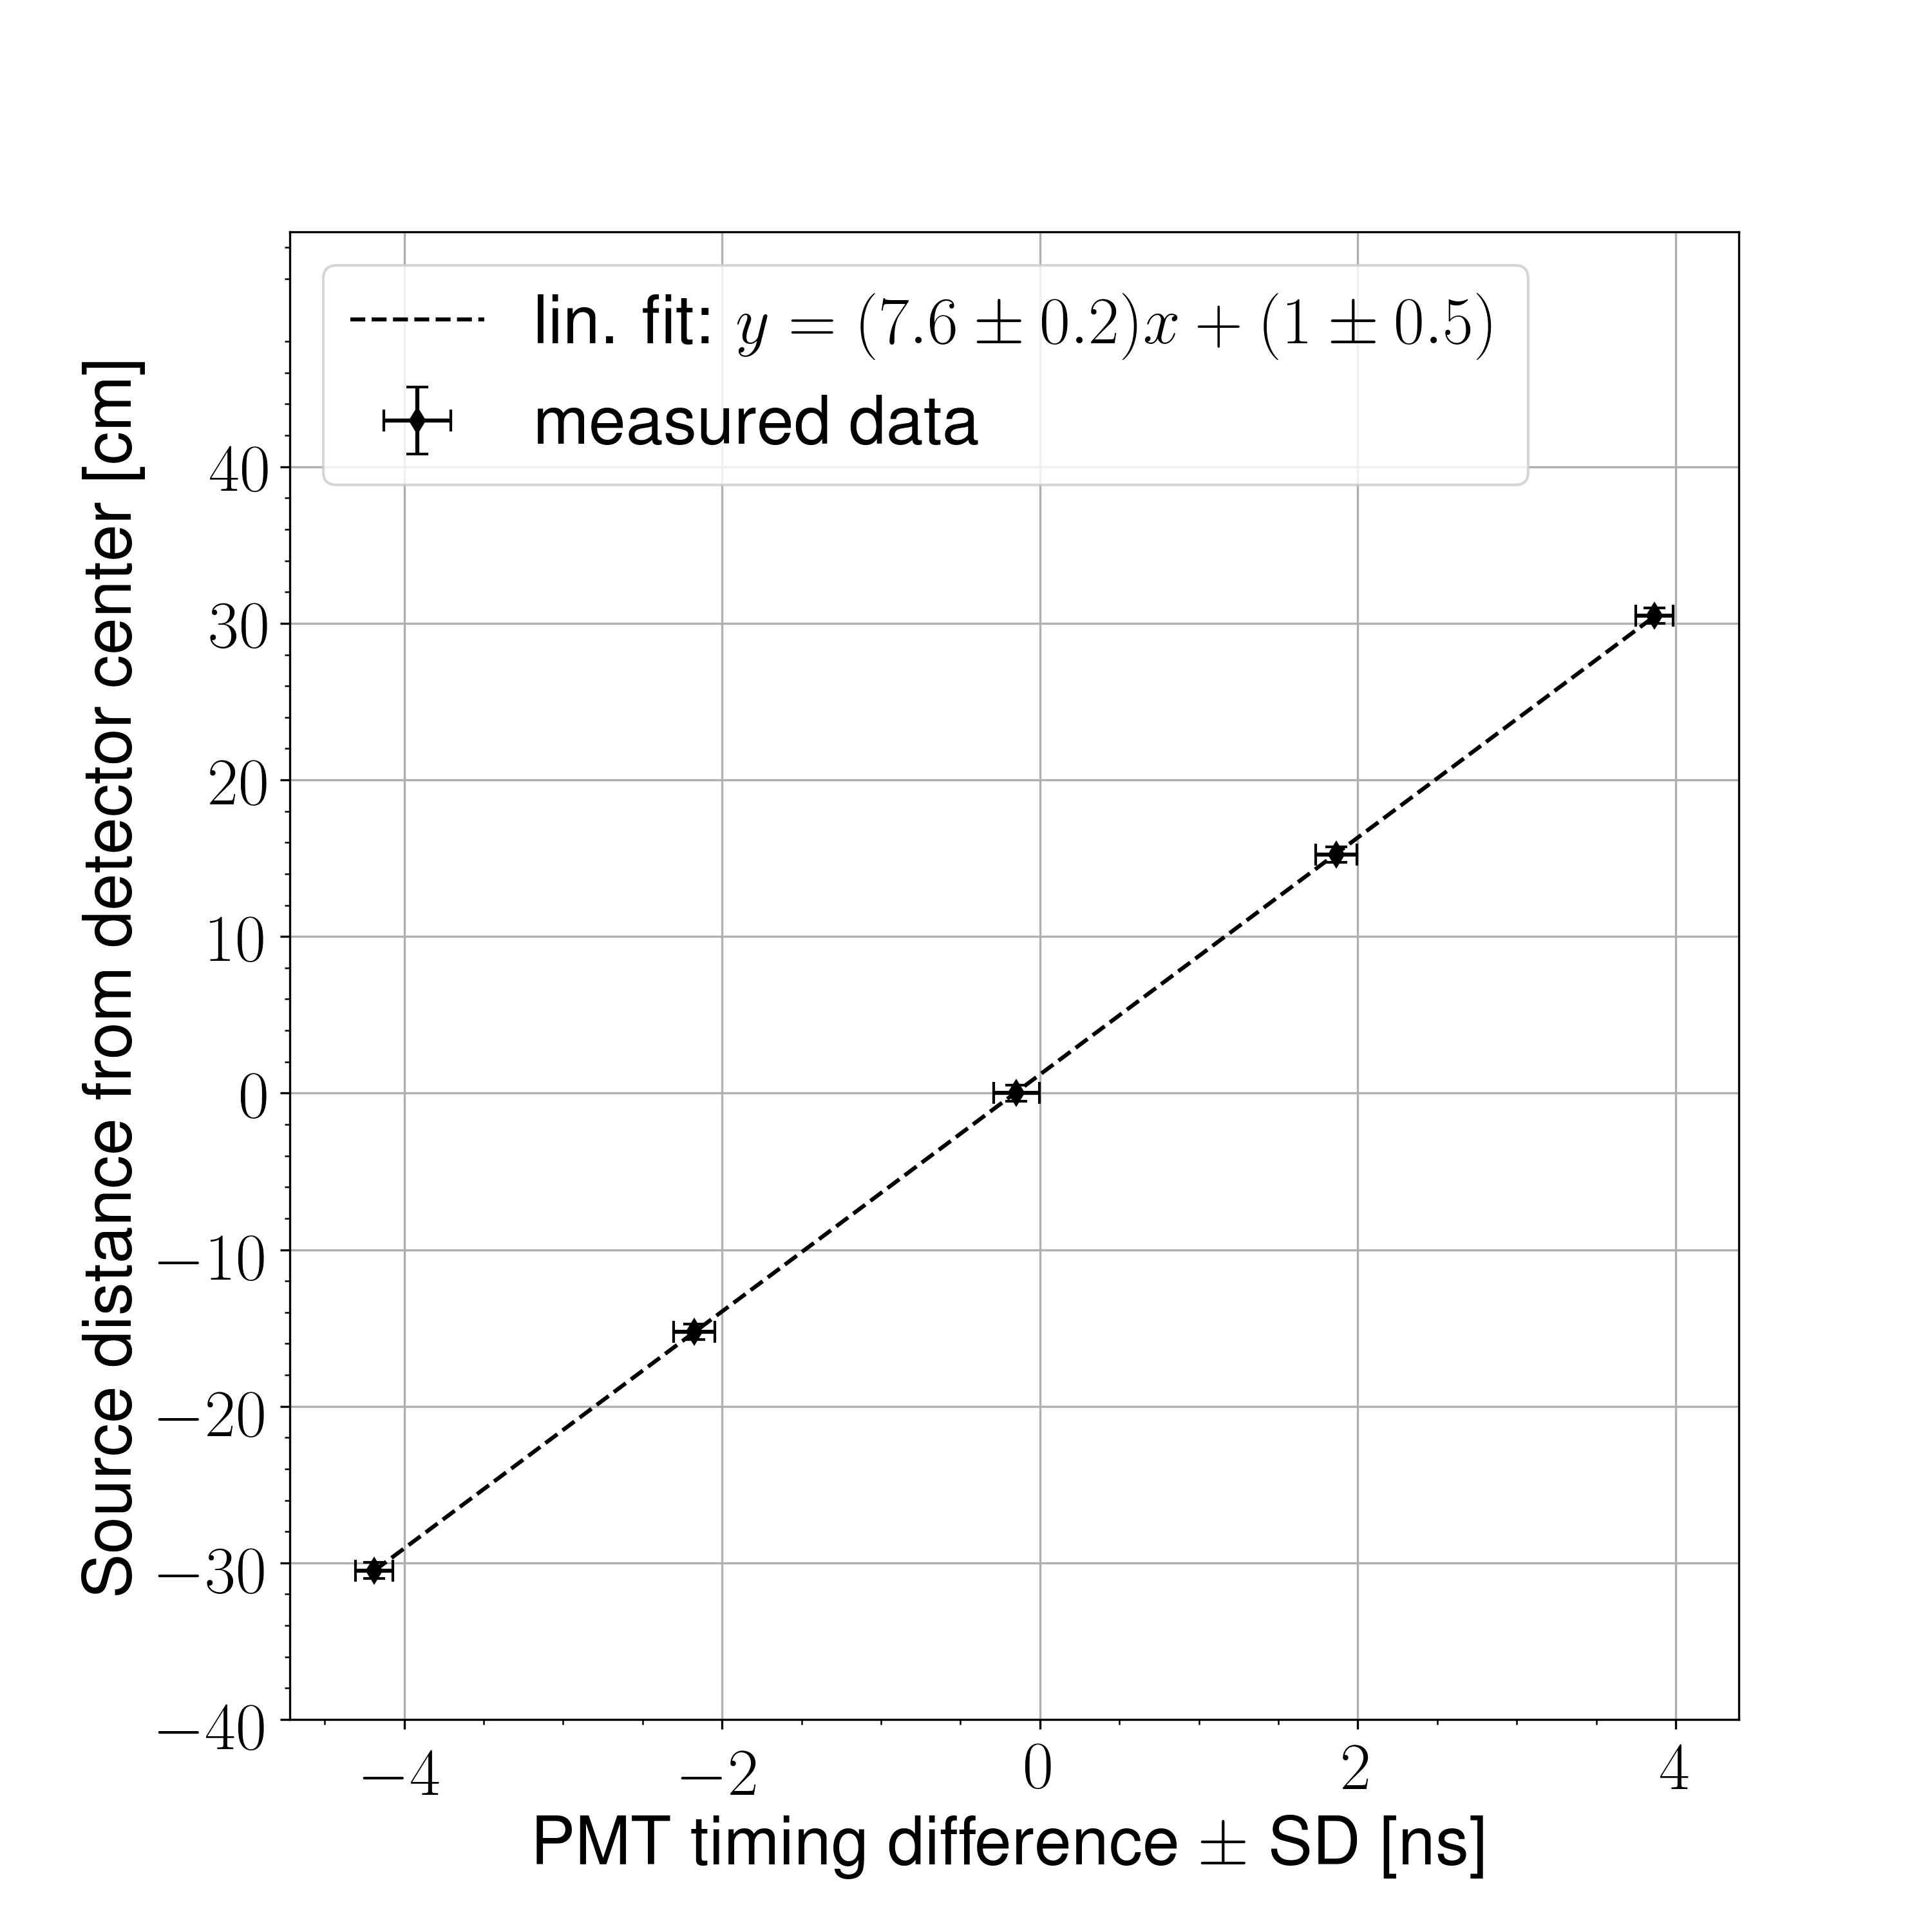
\includegraphics[width = 0.9\textwidth]{Content/Methods/PMTDifference.png}
    \caption{A collimated $^{60}$Co source is used to produce events at precise locations on the detector.
    The particle's position along the detector's length is shown to vary linearly with respect to the timing difference between events in the top and bottom PMTs of a detector.}
    \label{fig:PMTDifference}
\end{figure}
\subsubsection{Discussion of Experimental Errors}
\label{Errors}
All sources of error can be classified into three groups: \begin{enumerate*}[font={\color{red!50!black}\bfseries}]
\item \textit{Resolution of measurement}, a source of random error cause by the finite precision of particle ToF and position determination,
\item \textit{Error in measured rates due to counting statistics}, also a source of random error, and
\item \textit{Systematic errors}.
\end{enumerate*}

\paragraph{Resolution of measurement}.
The position of a detected particle is known to within a specified resolution, which translates into a resolution in the measurement of the opening angle between a pair of particles.
The extent that positional resolution leads to a corresponding opening angle resolution depends on the value of the opening angle.

\paragraph{Counting error}.
The measured rate of a given opening angle is subject to the poissonian distribution.

\paragraph{Systematic errors}
% ToDo: Cross-talk discussion can go here. So can alastic acattering in teh target. BUT, elastic scattering may also be a resolution. hmm...
This study reports two-neutron opening angle distributions expressed by a ratio between a correlated distribution and an uncorrelated distribution in which the same set of neutron events are used to form both distributions.
This produces a result that is unaffected by several effects which would otherwise be large potential sources of systematic error, such as the absolute neutron efficiencies of each detector, drift in the high voltage supplied to the PMTs, and the geometrical acceptance of the detector array as a function of opening angle.
Furthermore, \textit{accidental} two-neutron events, which lead to an over estimation of the isotropic component of the opening angular distribution, are subtracted from the data.
\textit{Accidental} two-neutron events are defined as the detection of two causally uncorrelated events in the same pulse if both events occur during the neutron ToF window.
The subtraction of such events are possible under the assumption that the number of detected accidentals per pulse follows the poissonian distribution.
See section~\ref{Analysis} for a detailed discussion on how this is accomplished.
The validity of this assumption can be tested with measurements taken while using D2O as a target.
All coincident neutrons from the photo-disintegration of deuterium are accidentals because only one neutron is produced per disintegration.
Figure~\ref{fig:PoissonianFits}a shows that a poissonian model produces a good fit to the distribution of the number of neurons detected in coincidence while using D2O as a target.
When using DU, there is the inclusion of correlated neutrons alongside any accidentals, so the poissonian model underestimates the rate.
\begin{figure}[htbp]
    \centering
    \subfloat[D2O target: high p-value, good compatibility.]{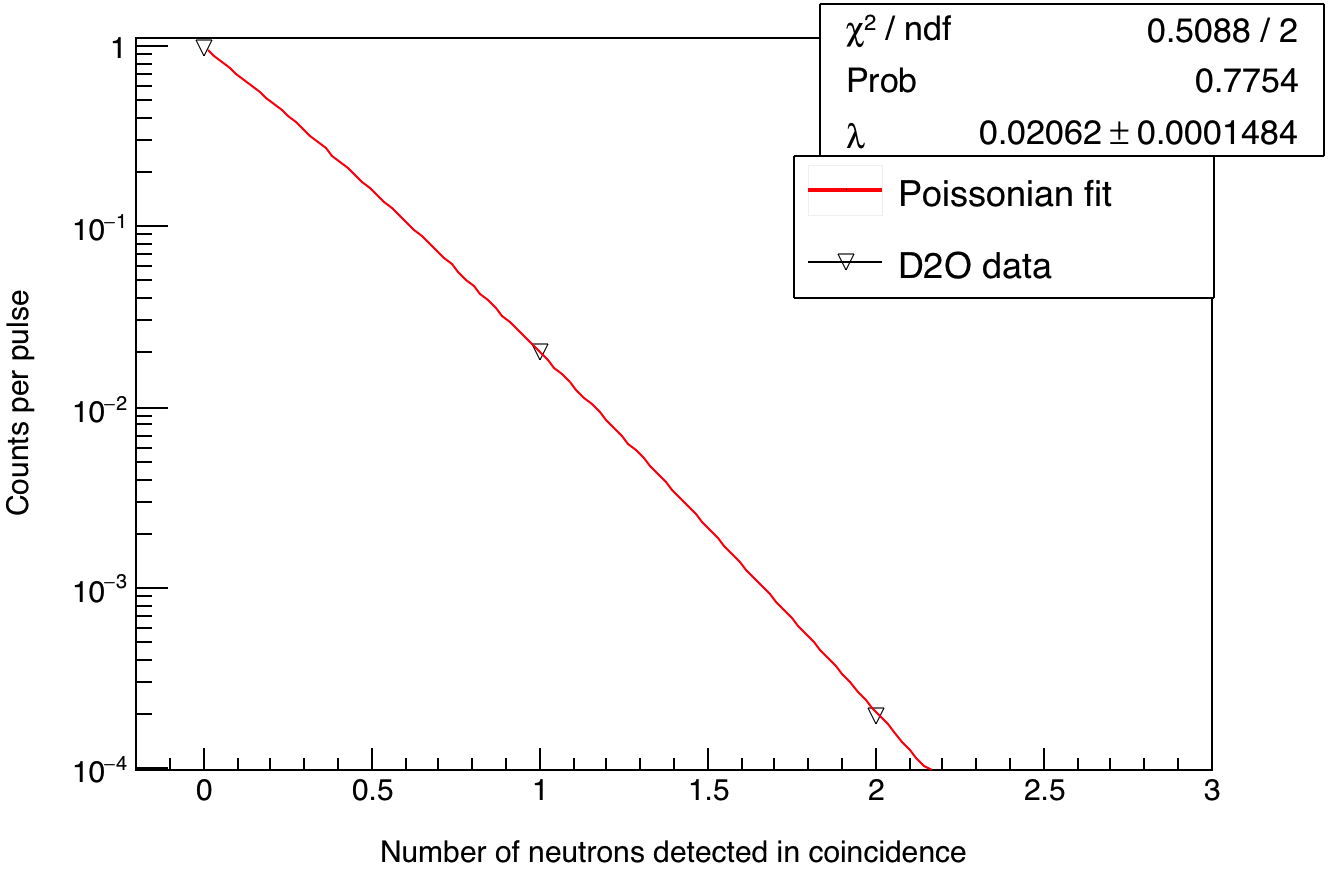
\includegraphics[width=0.55\textwidth]{Content/Methods/PoissonianFitD2O.png}}
    \subfloat[DU target: low p-value, poor compatibility.]{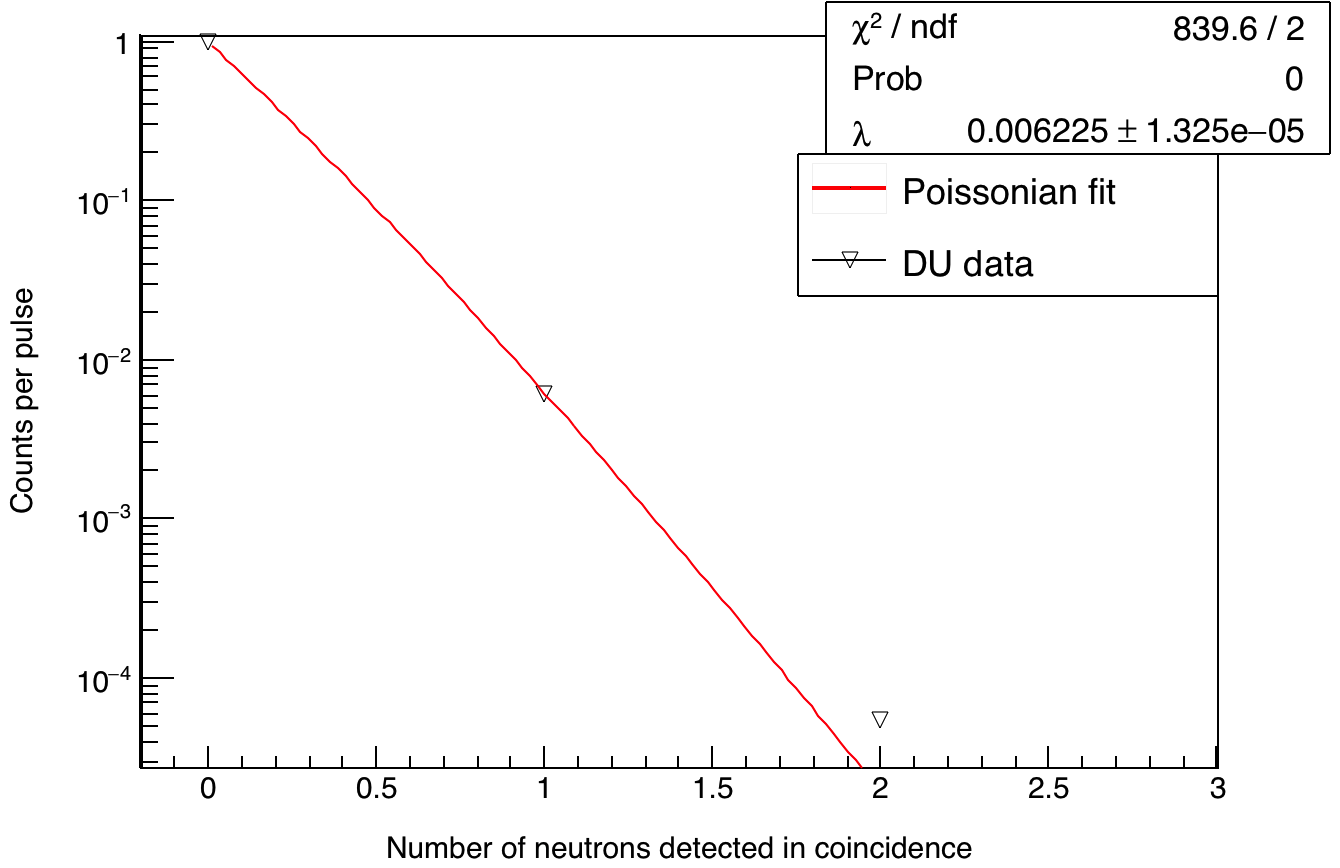
\includegraphics[width = 0.55\textwidth]{Content/Methods/PoissonianFitDU.png}}
    \caption{A D2O target (left) produces only accidental neutrons, so a poissonian model is suitable.
    The p-value, denoted 'prob' on the plot, is a metric for assessing the compatibility of the data to a given model, poissonian in this case.
    A p-value of 0.77 for the D2O target indicates relatively good compatibility.
    When using DU as a target (right), both accidental and correlated neutrons are produced, so a poissonian model is not suitable.
    The assumption that accidentals themselves follow the poissonian distribution is used to subtract them from the data.}
    \label{fig:PoissonianFits}
\end{figure}
\begin{figure}[h]
    \centering
    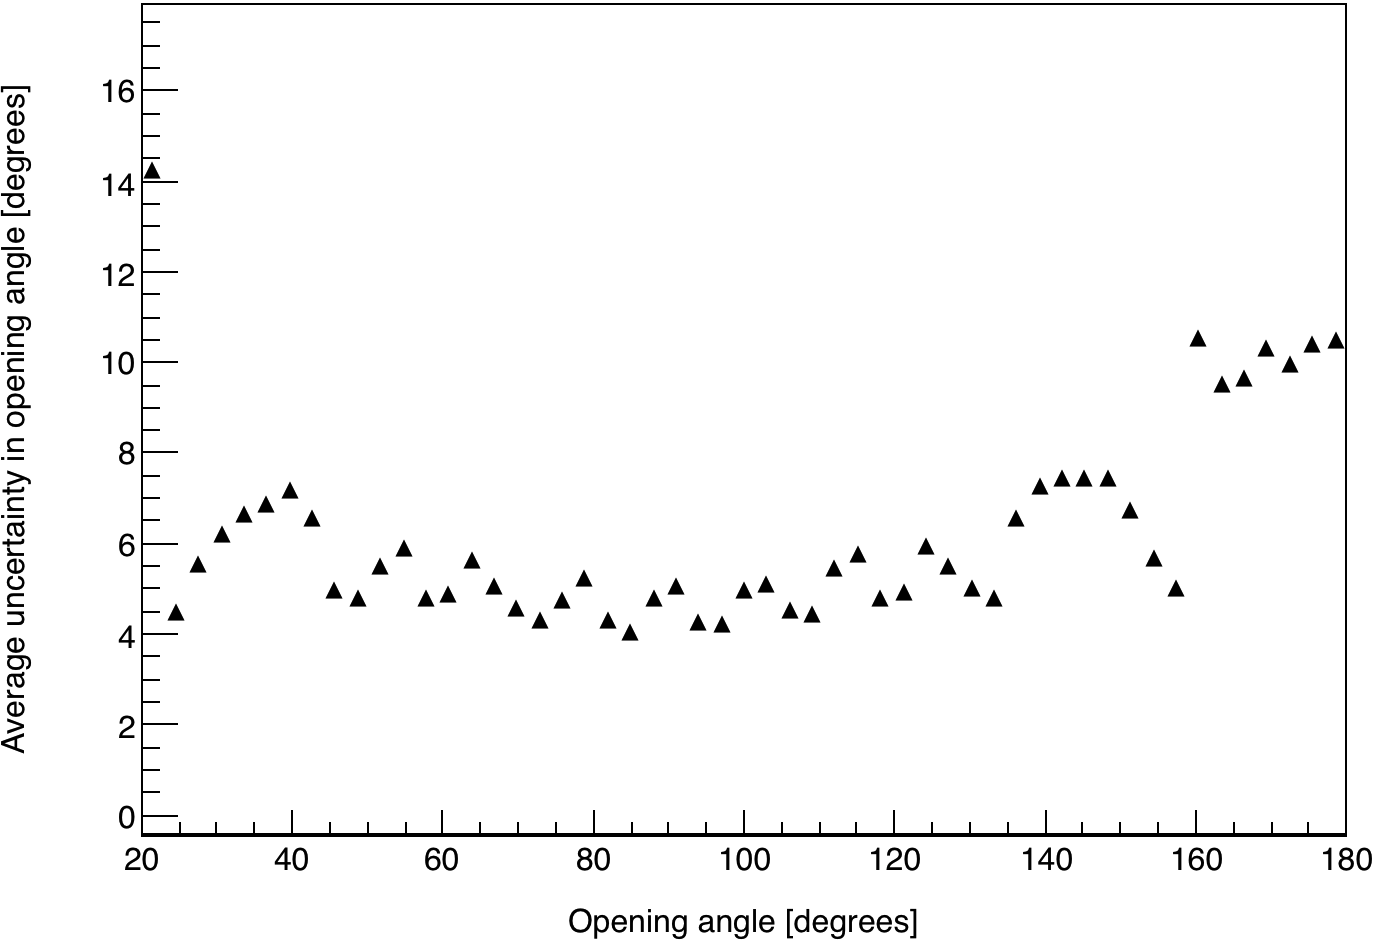
\includegraphics[width = 0.75\textwidth]{Content/Methods/OpeningAngleUncertainty.png}
    \caption{Uncertainties in opening angle as determined by the propagation of position uncertainties through the opening angle calculation.
    Because the uncertainty of a given opening angle measurement varies depending on which two detectors are involved, an average of the calculated uncertainties of measurements falling within each bin is taken.
    The y-axis can be viewed as a measure of the angular resolution in the sense that it represents the smallest angular difference that can be considered statistically significant.
    }
    \label{fig:CrossTalkExamplepng}
\end{figure}

\subsubsection{Detector Shielding}
The detector's shielding was designed with the aim of reducing cross-talk, the detection of photons, and noise.
The front face of the detectors, which face towards the target, are subject to the highest flux of gammas due to the scatting beam photons from the target.
The detection of a gamma renders a detector ``dead'' during the time in which fission neutrons reach the detectors.
Lead readily attenuates gammas, but has the side effect scattering neutrons.
If a neutron scatters prior to being detected, the ToF calculation will be incorrect because the neutron traveled an unknown distance to the detector.
The extent to which neutron distances of travel are perturbed due to scattering from lead shielding was quantified using an MCNP .
% ToDo: Add figure of neutron position variance cause by lead scattering.
Accordingly, 1" of lead was placed along the front face of the detectors.
This effectively diminished gamma detection rates and, according to the simulation, is expected to cause negligible levels of neutron scattering.
Additional lead was used in some special areas that had high gamma flux: at the sides of detectors adjacent to the beam, and along the front faces of the detectors farthest downstream.
Placing lead behind the detectors was avoided in consideration of an MCNP-POLIMI simulation, which indicated that lead placed here facilitates cross-talk.
Because cross-talk events are in fact correlated, they cannot be removed in analysis by the subtraction of accidentals.
For more information about cross-talk, see section~\ref{crosstalk}.

\subsection{Detector Cross-talk}
\label{crosstalk}
%**ToDo: The cross-talk plot on the wiki might be insightful.
\textit{Cross-talk} is an undesirable phenomenon that occurs when a particle is detected in one detector, and then by any means (e.g.\ elastic scattering), the same particle is detected in a different detector.
If both detections occur within the time frame typical for neutrons, then the cross-talk event cannot be distinguished from a true neutron coincidence.
The geometry of the neutron detector array makes it kinematically impossible for a neutron to scatter from a proton in one detector--which is the basis for scintillation--and then travel directly to another detector with enough kenetic energy to be detected.
Rather, in order for cross-talk to occur, it is kinematically required that the neutron scatter from at least one intermediate nucleus while traveling between detectors.
This fact, which can be derived from the conservation of energy and momentum, makes cross-talk a "second-order" effect, because upon depositing enough energy to be detected in one scintillator, the neutron must then 1) scatter from an intermediate nucleus, and 2) be detected in a second detector.
\begin{figure}
    \centering
    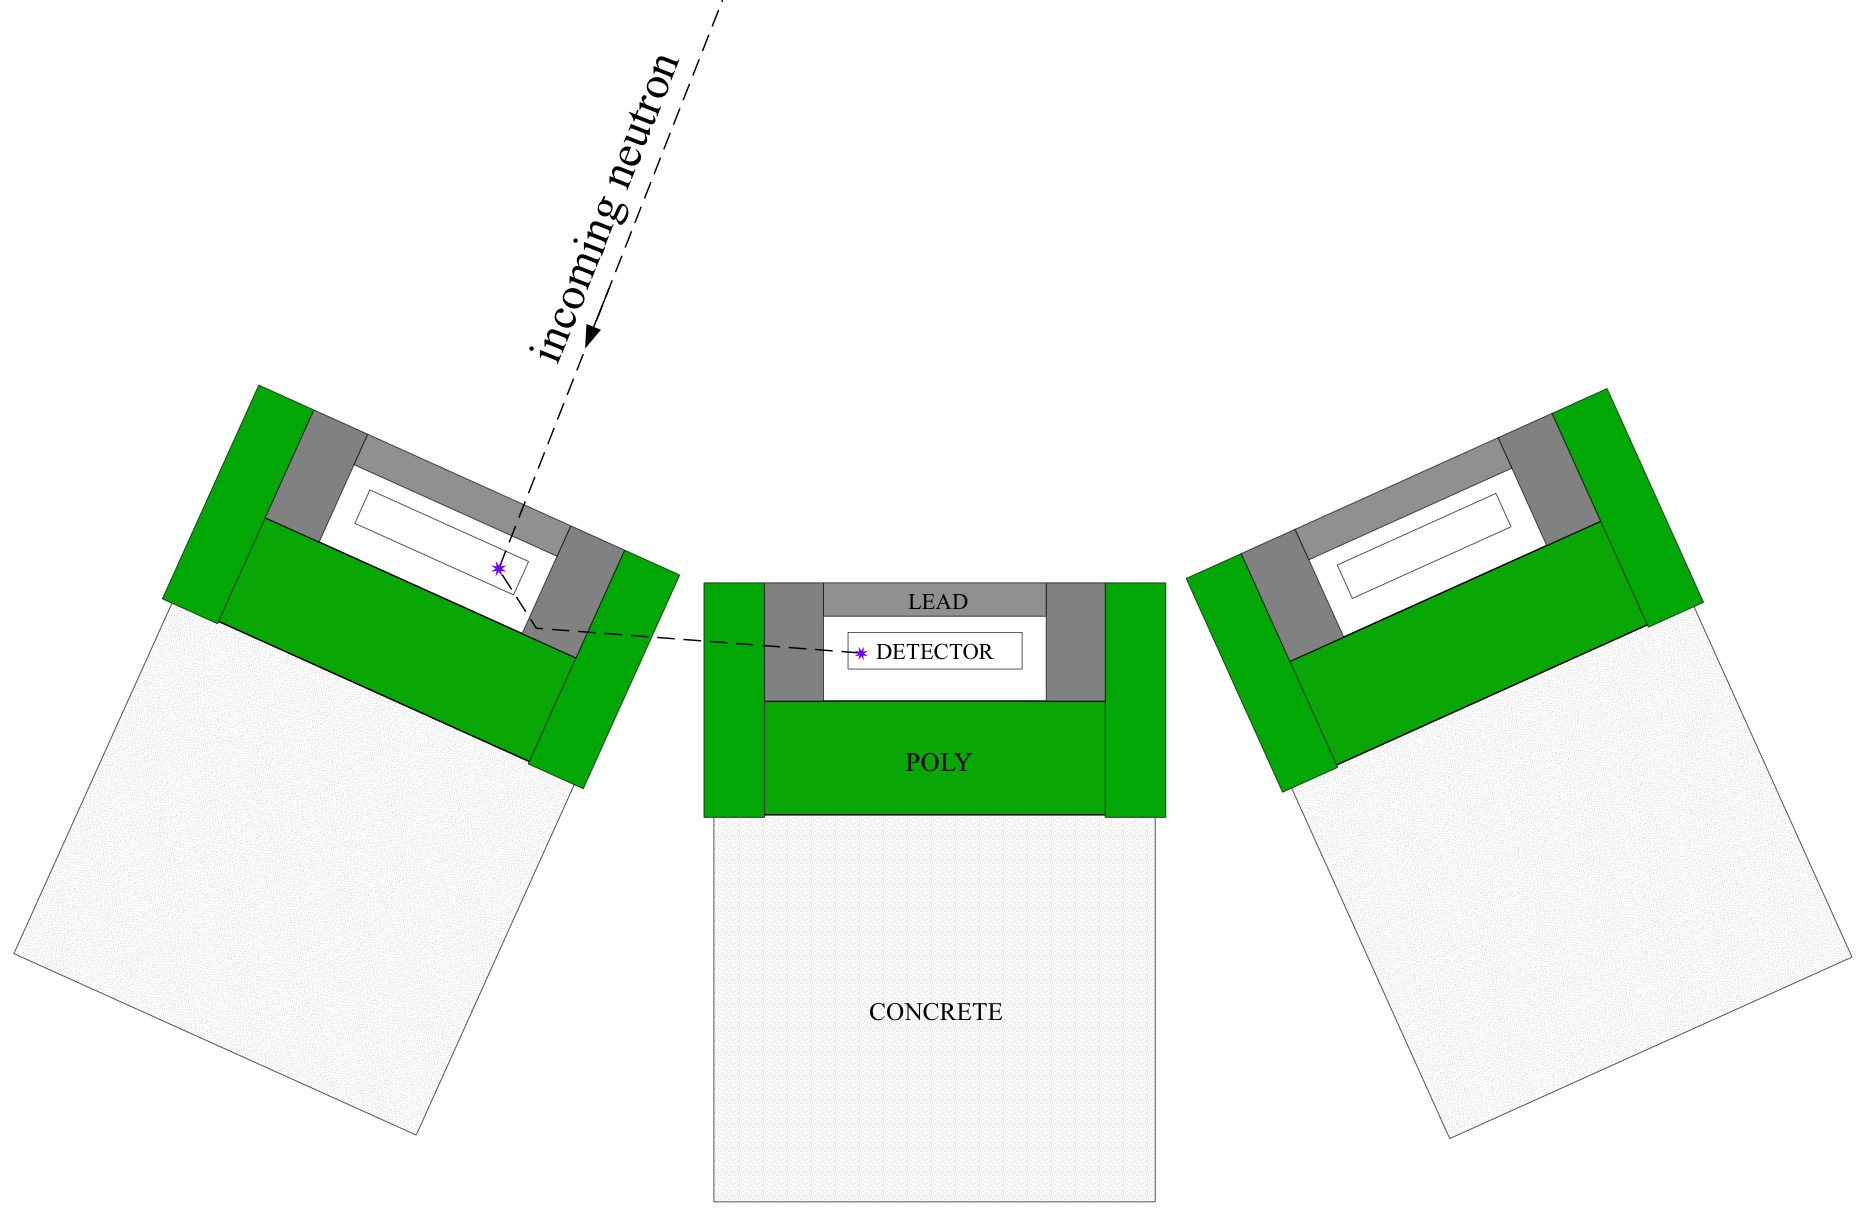
\includegraphics[width = 0.75\textwidth]{Content/Methods/CrossTalkExample.png}
    \caption{A hypothetical example of a neutron cross-talk event.
First, an incoming neutron enters a detector and is detected as the result of a collision with a proton.
Next, it scatters from some lead shielding nearby, which changes its direction of travel such that it enters a second detector where it is detected a second time.
The scattering of a neutron from an intermediate nucleus, in this case a lead nucleus in the detector's shielding, is kinematically required in order for cross-talk to occur in this experiment.}
    \label{fig:CrossTalkExamplepng}
\end{figure}
However, The fact that cross-talk is a second-order effect is not sufficient to make the claim that cross-talk is negligible,
because the detectors and their shielding contain significant levels of carbon, lead, and other nuclei which could function as intermediate scattering points.
To address this, a detailed MCNP-PoliMi simulation was performed that includes the entire array of neutron detectors, along with their shielding, supporting structures, and the concrete composing the experimental cell which contains the detectors.
PoliMi is an extension to MCNP that was developed to simulate correlated fission particles and their subsequent interactions as accurately as possible.
PoliMi includes multiplicity distributions for neutrons, photons, and the correct correlated photon production from neutron interactions.
These features are in contrast to the standard release of MCNP which uses uncorrelated distributions and average multiplicities.
As a result, the standard release of MCNP converges to the correct average result quicker than if correlated event-by-event distributions were used.
Another feature PoliMi provides is the ability for particle tracking data to be printed and post processed by the user.
Here, the particle tracking data is used to model detector physics in order to estimate the ratio of the rate of cross-talk to the rate of the detection of correlated neutrons.
Neutron detection physics was modeled by converting the amount of energy deposited by neutrons into scintillation light output, and did not include the propagation or detection of scintillation light.
The scintillation light output is given in MeV equivalent electron energy, denoted MeVee.
Neutron energy deposited from collisions with hydrogen and carbon nuclei is the only input used to calculate light output, the procedures of which are taken from ref~\cite{POLIMI}.
For neutron collisions with hydrogen, the light output is given by
\begin{displaymath}
L = 0.0364 E_n^2 +  0.125 E_n
\end{displaymath}
where $E_n$ is equal to the change in the kinetic energy of the neutron during the collision.
Neutron interactions with carbon are assumed to generate a smaller light output of
\begin{displaymath}
L = 0.02 E_n
\end{displaymath}
The simulation used MCNP-PoliMi's built in $^{252}$Cf spontaneous fission source, which emits neutrons with the correct correlations.
The light output threshold for detection was set empirically by choosing the threshold that gave the best agreement between the ToF spectra of simulation and measurement (see fig~\ref{fig:Cf252MCNPVsEXP}).
\begin{figure}
    \centering
    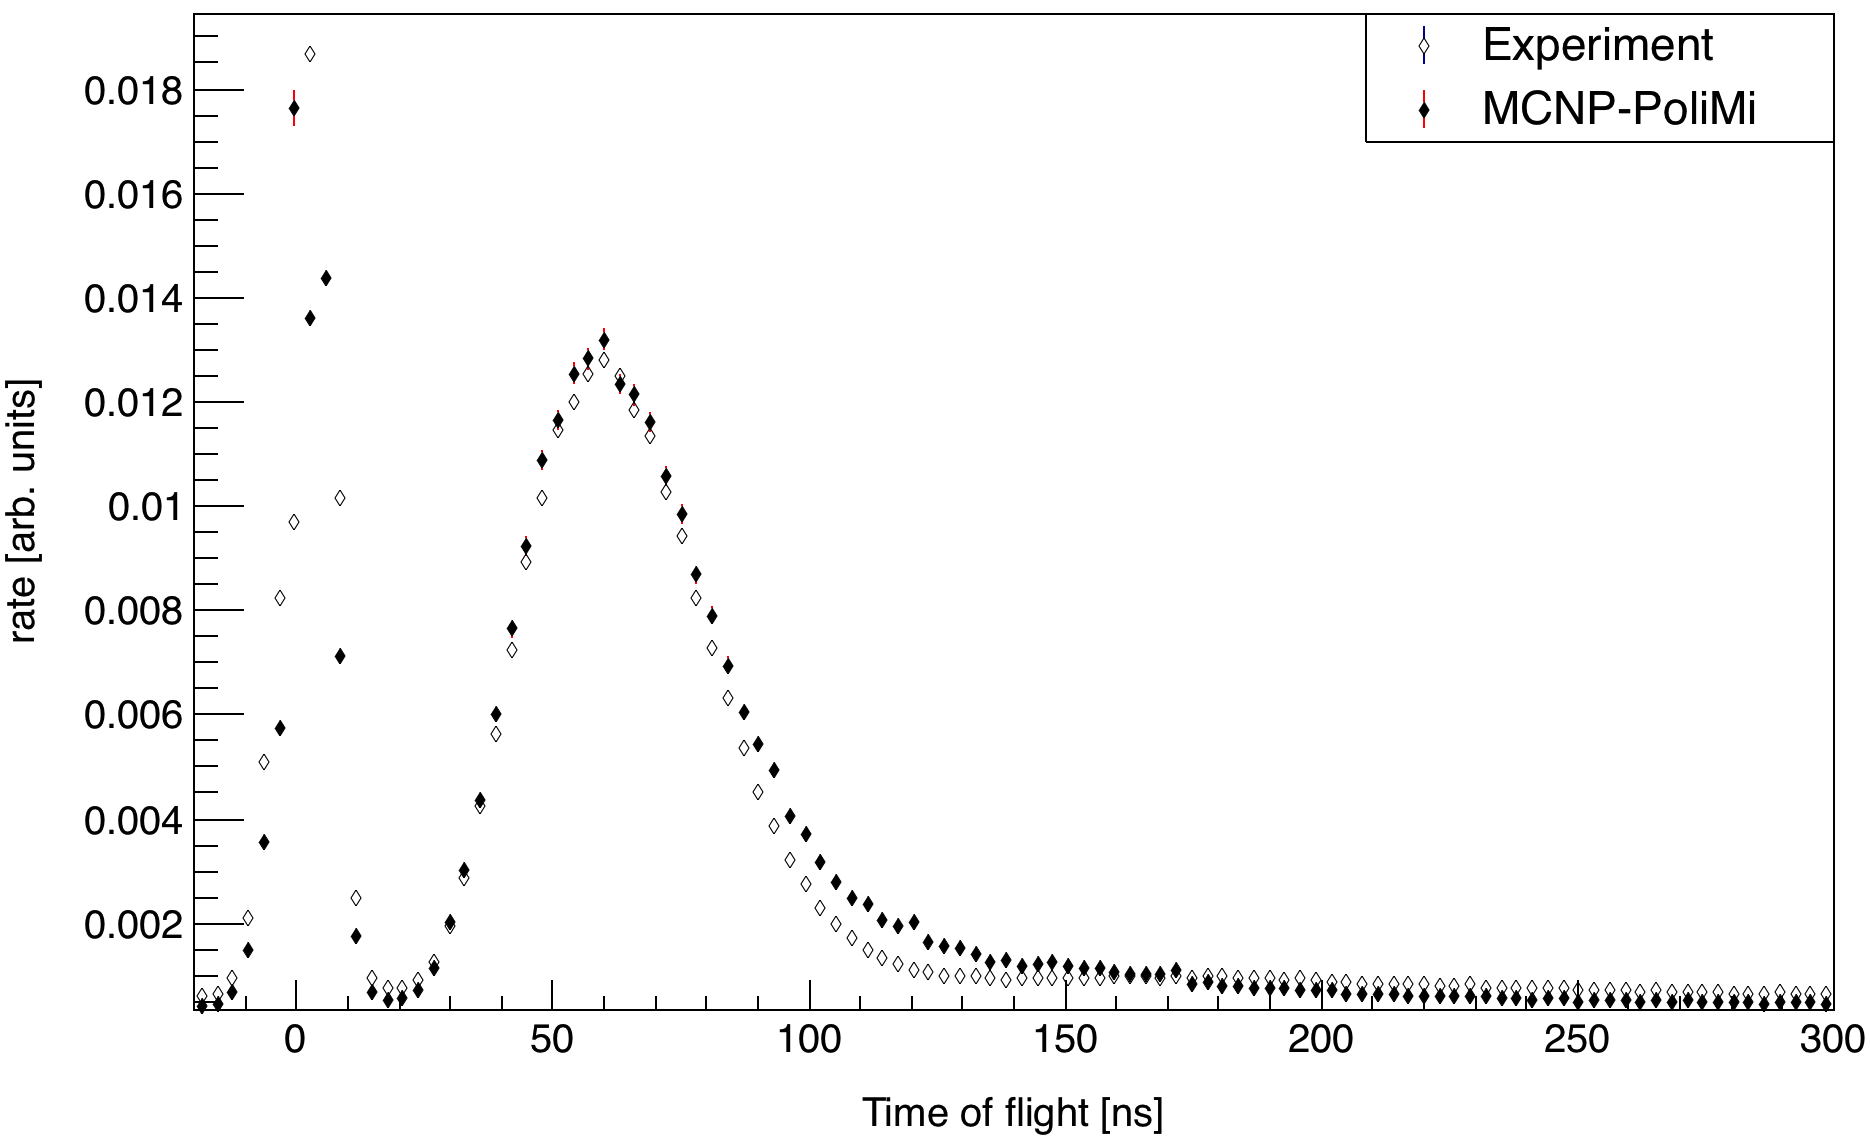
\includegraphics[width = 0.9\textwidth]{Content/Methods/Cf252MCNPVsEXP.png}
    \caption{Measured vs simulated ToF spectrum of a $^{252}$Cf spontaneous fission source.
    In the simulation, the light output threshold for detection was chosen by varying it until good agreement with measurement was achieved.}
    \label{fig:Cf252MCNPVsEXP}
\end{figure}
A tally is kept of number of cross-talk events and the number of correlated neutron pairs detected.
An event is considered a "neutron event" if there is a light output of greater than 0.03 MeVee produced in a detector in a time frame of 10 ns or less.
Furthermore, the 0.03 MeVee light output threshold must be reached sometime during the neutron time of flight window used in the experiment, which is 45 to 150 ns.
This way, the method used for particle identification in the simulation mimics that which is used in the experiment.
In the simulation, cross-talk events accounted for 3\% of total correlated events.
Accordingly, no cross-talk corrections were applied to the data.

\subsection{Targets}
A depleted uranium (DU) target with dimensions of 4x2x0.05 $\text{cm}^3$ was used as the primary target for the measurement of two-neutron correlations.
DU received the majority of the allotted beam time because it is an even-even nucleus and as a consequence the fission fragments are emitted with a high degree of anisotropy.
One consideration for the design of the target is the rate at which neutrons produced in the target scatter before exiting.
This is a cause for concern because a neutron's direction of the travel is altered by scattering, which creates two-neutron opening angles that are not reflective of the opening angle immediately after fission.
This effect cannot be completely eliminated, so the target must be small enough such that neutron scattering is negligible.
The size of such a target is found by performing an MCNP simulation in which neutrons with an energy spectrum typical of fission neutrons are sampled uniformly within the target.
From the simulation, 97.5\% of the neutrons produced in a 4x2x0.05 $\text{cm}^3$ DU target escaped without scattering.
Because two neutrons are required for the formation of an opening angle, the rate of data contamination due to scattering would be $(1-.975^2)$, or 5\% of two-neutron events.
% ToDo: Expand on this section a little bit. Add the plot of contamination VS radius.
\begin{figure}
    \centering
    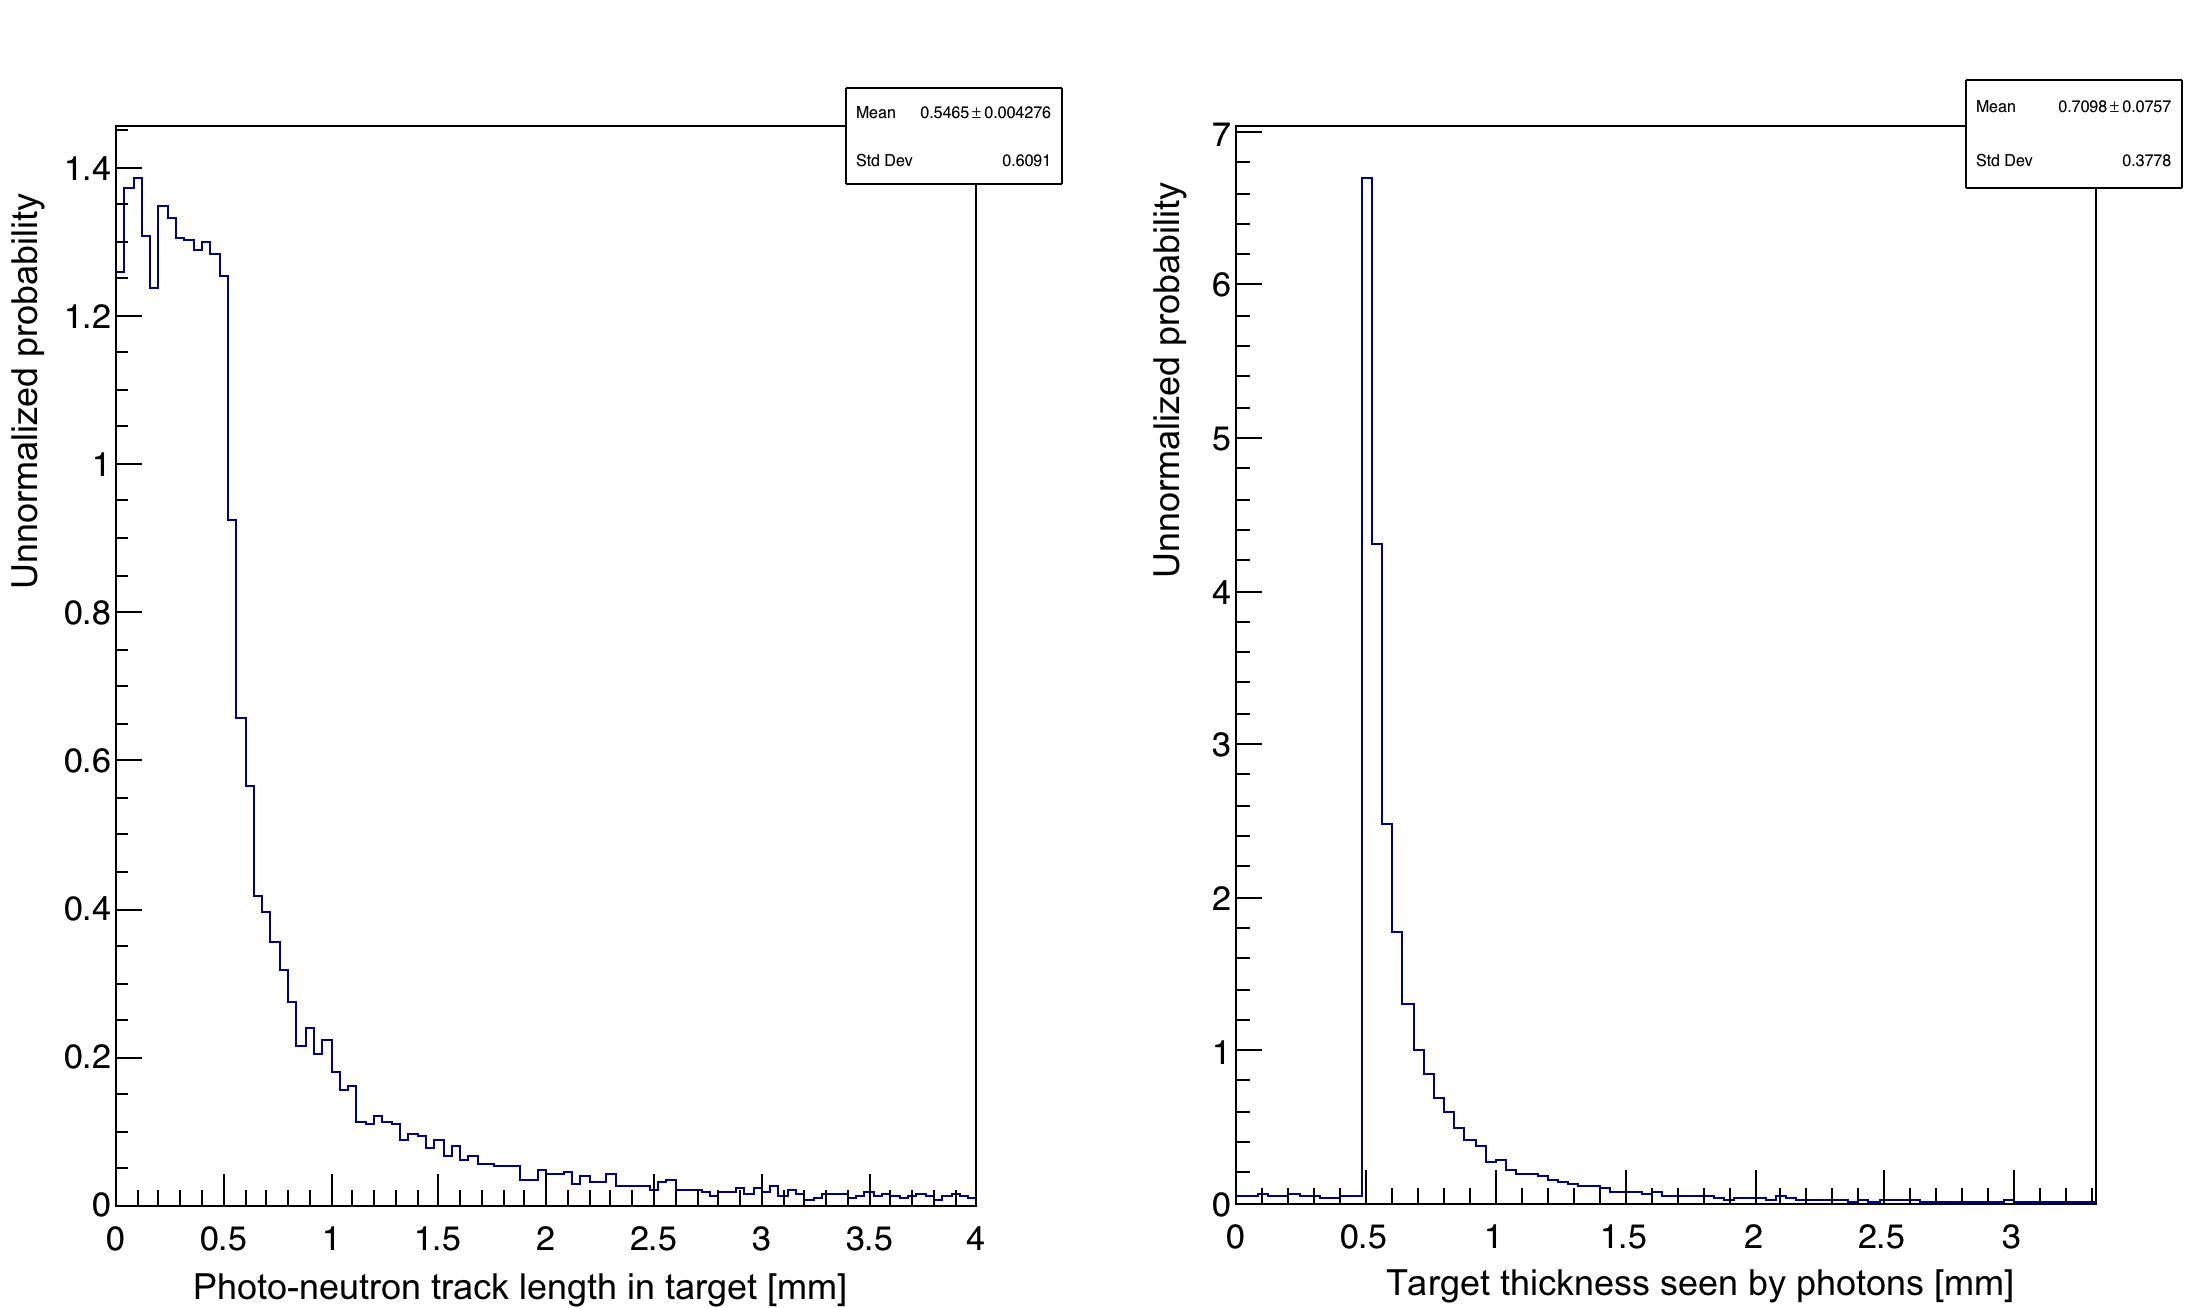
\includegraphics[width = \textwidth]{Content/Methods/ScatteringInTarget.png}
    \caption{}
    \label{fig:ScatteringInTarget}
\end{figure}

It is desirable to have a target with symmetry that is consistent with the cylindrical symmetry of the neutron detector array.
To accomplish this, a thin rectangular target was rotated slowly about the vertical axis during data acquisition.
By doing this the cylindrical symmetry is preserved, since the measurement is reflective of an average of events which occurred while the target was at orientations from 0 to 2$\pi$.
This eliminates potential biases caused not by physics, but instead by the asymmetrical structure of the target.

\subsection{Measurements with $^{252}$Cf}
%ToDo: Place our results of Cf measurements here in comparison to past measurements.

Opening angle measurements were also performed on neutrons from the spontaneous fission (SF) of $^{252}$Cf.
The configuration for this was different than that for photofission measurements, as the photon beam can no longer be used for the timing of a ``start'' trigger.
The trigger for $^{252}$Cf consisted of two high timing-resolution scintillation photon detectors, where one is fixed below and the other above the source at a distance of 15 cm.
Using a coincidence window of 4 ns, the timing start trigger required 2-fold coincidence between both the photon detectors.
Aside from a different mechanism for a start trigger, the methods used for the measurement of two-neutron opening angle distributions in the SF of $^{252}$Cf are equivalent to those used for photofission.

As opposed to the measurements of neutrons from photofission, there is no concern over the detection of accidental neutron pairs because given the strength of the $^{252}$Cf source, it is highly unlikely for two fissions to occur during the neutron time of flight window.
Another difference between the two measurements is the clean and sharp peak produced by fission photons from $^{252}$Cf, compared to a relatively smeared peak produced by photons scattering from the target during measurements of photo-neutrons.
In each measurement, the photon peak is used as a reference point for the calculation of neutron ToF.
As a result the $^{252}$Cf measurements have less error in ToF caused by the spreading of the photon peak used for reference.
The same normalization technique is used for both measurements, in which the correlated distribution is divided by the uncorrelated distribution of neutron pairs taken from different fissions.
There is good agreement among past measurements of the opening angle distribution of neutrons from the spontaneous fission of $^{252}$Cf, and so they serve as a good benchmark for the quality of measurements performed in this study.


